\chapter{Integration der Algorithmen} \label{Kap4}

In diesem Kapitel werden die zuvor beschriebenen Kartierungsalgorithmen in das eigene Package integriert. Dazu werden die Algorithmen als ROS-Packages installiert, durch das eigene Package konfiguriert und mittels eines Launch-Files gestartet.

Das Ziel jeder Integration in das Package ist das Online-\ac{SLAM}, bei dem die Karte während der Aufnahme erstellt wird, als auch das Offline-\ac{SLAM}, bei dem die Karte erst nach der Aufnahme berechnet wird.

\section{Aufsetzen des eigenen Packages}

Um den Roboter nun nutzen zu können, muss dieser mit dem Robot Operating System verbunden werden. Dazu werden einige Packages benötigt, die in einem selbst entwickelten Package zusammengefasst werden.

\begin{itemize}
  \item \textit{p2os:} Dieses Paket stellt die Schnittstelle zur Hardware des Pioneer 3-DX zur Verfügung. Das Package bietet daneben noch die Steuerung mittels Tastatur oder Joystick.
  \item \textit{sicktoolbox\_wrapper:} Dieses Paket startet den Laserscanner Sick LMS und sendet die Scan-Daten an einen Topic.
  \item \textit{ROS-tinkerforge\_sensors:} Dieses Paket startet die Inertial Measurement Unit Tinkerforge Brick 2.0 und sendet die Beschleunigungsdaten an einen Topic.
\end{itemize}

Das eigene Package hat den Namen pioneer3dx\_cartographer und ist in folgende Ordner eingeteilt:

\begin{itemize}
  \item \textit{launch:} Dieser Ordner beinhaltet alle Launch-Files.
  \item \textit{defs:} Dieser Ordner stellt das Xacro-Modell des Pioneers zur Verfügung.
  \item \textit{meshes:} Dieser Order stellt die geometrischen Informationen des Pioneers als STL-Dateien zur Verfügung.
  \item \textit{configuration\_files:} Dieser Order speichert Konfigurationen für den RVIZ oder für Algorithmen.
\end{itemize}

Im ersten Schritt ist im Launch-Ordner die Datei pioneer.launch von Bedeutung, da dieses den Motor, den Laserscanner und die Intertial Measurement Unit des Pioneers, sowie das Xacro-Modell und die benötigten Transformationen startet bzw. lädt. Im weiteren Verlauf des Kapitels wird der Ordner um weitere Launch-Files erweitert, die die einzelnen Kartierungsalgorithmen starten.

Im nächsten Ordner liegt das Modell des Pioneers im Format XML Macros (xacro). Dieses wird zur Laufzeit in das Unified Robot Description Format (URDF) umgewandelt. Ein Modell besteht immer aus mehreren Links und Joints. Ein Link beschreibt einen Teil des Roboters, der Informationen über seine Trägheit und über das Aussehen definiert. Ebenfalls wird in einem Link ein Kollisionsmodell definiert. Links werden über Joints miteinander verbunden. Beispiele für einen Link sind die Räder oder die Basis des Roboters. Das Aussehen eines Links wird über geometrische Informationen im STL-Format definiert. Die STL-Dateien eines jeden Links liegen im Folder meshes. \autocite{xacroRosWiki} \autocite{urdfRosWiki}

Das Modell im xacro-Format lässt sich manuell in das urdf-Format umwandeln. Danach kann eine Grafik der Links und Joints per Kommando erstellt werden.

\lstinputlisting[language=Bash,caption={Umwandlung von xacro in urdf und grafische Darstellung},label=lst:ROSXacro,float=b]{\srcloc/ROS_Xacro-2-URDF.sh}

Für den Pioneer 3-DX ergibt sich dann die folgende Baumansicht in \autoref{Kap2:Pioneer3DXURDF} nach dem Ausführen von \autoref{lst:ROSXacro}.

\begin{figure}[t]
  \centering
  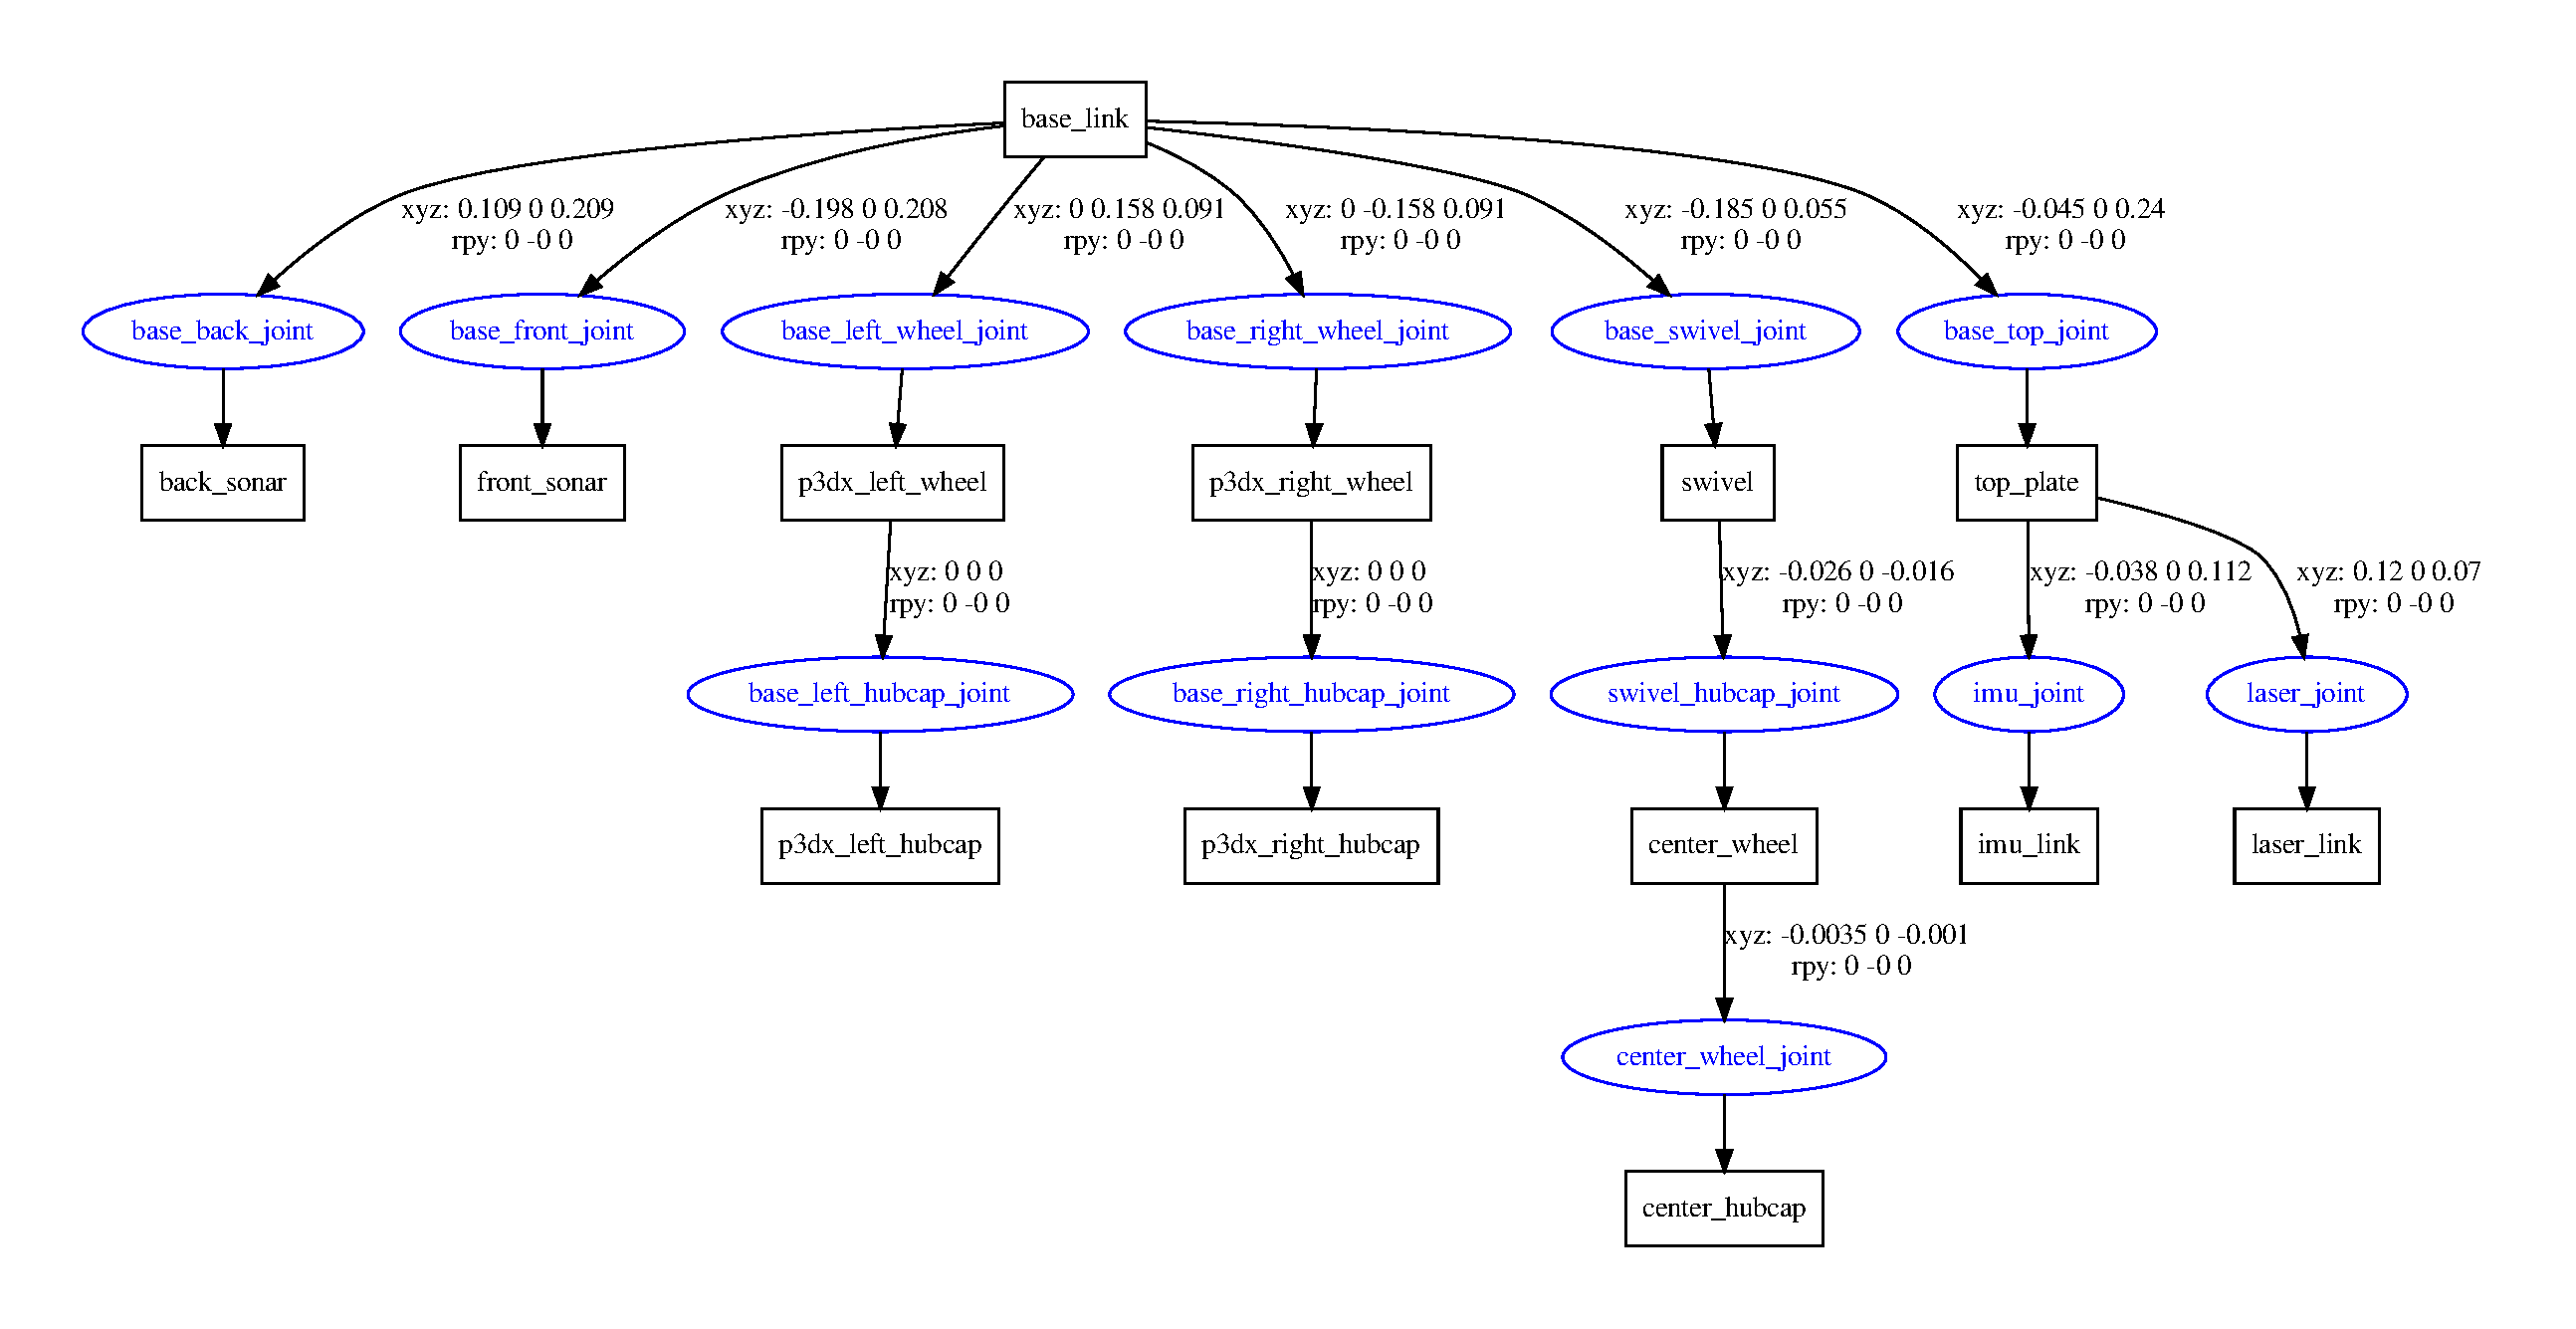
\includegraphics[width=14cm]{kapitel2/pioneer3dx_urdf}
  \caption{Pioneer 3-DX URDF-Modell}
  \label{Kap2:Pioneer3DXURDF}
\end{figure}

\section{Installation der Kartierungsalgorithmen}

Um das eigenen Package um die Kartierungsalgorithmen zu erweitern, müssen die Packages für die Kartierung installiert werden.

\subsection{cartographer}

Für die Installation des Cartographers müssen zunächst einmal die Paketquellen aktualisiert werden. Dann wird das Tool wstool sowie rosdep und Ninja installiert. Danach wird zum Catkin-Workspace gewechselt und einige weitere Installationsschritte mittels dem Tool wstool eingeleitet. Ist dieser Installationsschritt ausgeführt, muss jetzt mittels rosdep noch die Abhängigkeit hinzugefügt werden. Zuletzt muss der Build gestartet werden und der Cartographer installiert werden. Dabei wird das Tool Ninja genutzt, um den Build-Prozess zu verschnellern. \autocite{cartographerInstallation}

\lstinputlisting[language=Bash,caption={Installation des Packages Cartographer},label=lst:ROSCARTOGRAPHERINSTALL,float=t]{\srcloc/cartographer_installation.sh}

\subsection{hector\_mapping}

Die Installation des Packages hector\_mapping gestaltet sich wesentlich einfacher als die des Packages cartographer, da dieses manuell gebaut werden musste. Bei diesem Package wird lediglich der \ac{ROS}-Befehl zur Installation ausgeführt, wie in \autoref{lst:ROSHECTORMAPPINGINSTALL} dargestellt.

\lstinputlisting[language=Bash,caption={Installation des Packages hector\_mapping},label=lst:ROSHECTORMAPPINGINSTALL,float=t]{\srcloc/hector_mapping_installation.sh}

\subsection{gmapping}

Die Installation des Packages gmapping gestaltet sich ebenso einfach wie die des Packages hector\_mapping. Bei diesem Package wird wieder lediglich der \ac{ROS}-Befehl zur Installation ausgeführt, wie in \autoref{lst:ROSGMAPPINGINSTALL} dargestellt.

\lstinputlisting[language=Bash,caption={Installation des Packages gmapping},label=lst:ROSGMAPPINGINSTALL,float=t]{\srcloc/gmapping_installation.sh}


\section{Aufsetzen der Launch-Files und der Konfiguration}

Im nächsten Schritt werden die Launch-Files sowie damit auch die Konfiguration der Kartierungsalgorithmen aufgesetzt. Dabei muss berücksichtigt werden, dass für jeden Algorithmus andere \ac{ROS}-Nodes gestartet und andere Anforderungen an das Transformations-Modul TF erfüllt werden müssen, wie in \autoref{rosVerwendungCartographer},  \autoref{rosVerwendungHectormapping} sowie in \autoref{rosVerwendungGmapping} beschrieben. Pro Algorithmus wird sowohl ein Launch-File für die Online-Kartierung als auch eines für die Offline-Kartierung präsentiert. Bei ersterem wird die Karte während der Aufnahme erstellt. Bei zweiterem wird erst nach der Aufnahme das Bag-File an das Launch-File gegeben und somit wird erst im Nachhinein die Karte erstellt.

Allgemein enthalten alle Launch-Files zusätzlich den Startbefehl für den RVIZ, welcher als Argument eine Konfigurationsdatei enthält. Die Konfigurationsdatei beschreibt die Oberfläche des RVIZ.

\subsection{cartographer}

Der Cartographer definiert für das Online-Kartieren in \autoref{lst:ROSCARTOGRAPHERLAUNCHONLINE} eine Node, welche den Pioneer startet sowie zwei spezifische Nodes für den Cartographer. Die erste Node erhält als Argument eine Konfigurationsdatei, siehe \autoref{lst:ROSCARTOGRAPHERCONFIG}, mit Optionen zum Customizing der Cartographer-Node. Der zweiten Node wird lediglich die Auflösung der resultierenden Karte mitgegeben.

Die Konfigurationsdatei in \autoref{lst:ROSCARTOGRAPHERCONFIG} definiert die genutzten Frames und Nodes, die Frequenz sowie das Sampling von Daten. Dabei waren einige vom Standard abweichende Anpassungen nötig. Wenn eine IMU genutzt werden soll, muss das Attribut TRAJECTORY\_BUILDER\_2D.use\_imu\_data gesetzt werden. Die Anzahl der Laserscanner ist durch das Attribut num\_laser\_scans auf 1 gesetzt. Da 2D-Karten erstellt werden, muss das Attribut publish\_frame\_projected\_to\_2d aktiviert sein.

Das Launch-File für das Offline-Kartieren wird in \autoref{lst:ROSCARTOGRAPHERLAUNCHOFFLINE} gezeigt. Unterschiedlich zu \autoref{lst:ROSCARTOGRAPHERLAUNCHONLINE} ist, dass der Pioneer nicht mehr gestartet werden muss, sondern stattdessen beim Starten an das \ac{ROS}-Bagfile als Argument an das Launch-File übergeben wird, welches beim Start abgespielt wird.

\subsection{hector\_mapping}

Auch beim hector\_mapping in \autoref{lst:ROSHECTORMAPPINGLAUNCHONLINE} wird zunächst die selbe Node wie beim Cartographer definiert, die den Pioneer startet. In den weiteren Zeilen werden einige Konfigurationswerte definiert. Danach wird nur eine Node gestartet, welche diese Werte als Parameter nutzt. Die Konfiguration erfolgt also innerhalb des Launch-Files. In der Konfiguration werden unter anderem die Frames, die Auflösung, Größe und Position der Karte, einige Intervalle sowie der Topic für den Scan definiert.

Das Offline-Kartieren in \autoref{lst:ROSHECTORMAPPINGLAUNCHOFFLINE} erfolgt ähnlich wie das Online-Kartieren. Wie auch beim Cartographer muss das Launch-File des Pioneers nicht mehr gestartet werden. Stattdessen werden wieder die nötigen Nodes für das Einlesen des \ac{ROS}-Bagfiles genutzt.

\subsection{gmapping}

Auch beim gmapping in \autoref{lst:ROSGMAPPINGLAUNCHONLINE} wird zunächst die selbe Node wie beim Cartographer und beim hector\_mapping definiert, die den Pioneer startet. In den weiteren Zeilen werden ebenfalls wie beim hector\_mapping einige Konfigurationswerte definiert. Danach wird nur eine Node gestartet, welches diese Werte als Parameter nutzt. Die Konfiguration erfolgt also wieder innerhalb des Launch-Files. In der Konfiguration wird der Scan-Topic angegeben, sowie Parameter für die Maße und für das Erstellen der Karte.

Das Offline-Kartieren in \autoref{lst:ROSGMAPPINGLAUNCHOFFLINE} erfolgt wieder ähnlich wie das Online-Kartieren. Wie auch bei den anderen Kartierungsalgorithmen muss das Launch-File des Pioneers nicht mehr gestartet werden, sondern stattdessen nur die nötigen Nodes für das Einlesen des \ac{ROS}-Bagfiles.

\section{Starten der Kartierung}

Zum Starten der beschriebenen Online- oder Offline-Kartierungen, werden die gängigen \ac{ROS}-Befehle genutzt. Um diese folgenden Befehle ausführen zu können, muss der Anwender sich im Ordner des \ac{ROS}-Packages befinden.

\subsection{Starten der Online-Kartierung}

Die Online-Kartierung erfolgt immer über einen einzigen roslaunch-Befehl, welcher in \autoref{lst:ONLINE} dargestellt wird.

\lstinputlisting[language=Bash,caption={Online-Kartierung},label=lst:ONLINE,float=t]{\srcloc/online.sh}

\subsection{Starten der Offline-Kartierung}

Bei der Offline-Kartierung muss vorher ein Bag-File mit den gewünschten Topics aufgenommen werden, welches später einem Launch-File als Parameter übergeben wird. Dieses läuft wie in \autoref{lst:OFFLINE} beschrieben ab. Dieses Beispiel nimmt alle verfügbaren Topics auf. Es muss darauf geachtet werden, dass in einem zweiten Terminal das Launch-File des Pioneer vorher gestartet ist, damit Aktionen mit dem Roboter ausgeführt werden können.

\lstinputlisting[language=Bash,caption={Aufnahme eines Bag-Files},label=lst:OFFLINE,float=t]{\srcloc/offline.sh}

Nach der Aufnahme des Bag-Files, kann nun das eigentliche Erstellen der Karte ausgeführt werden. Dies läuft wieder über einen gängigen \ac{ROS}-Launch-Befehl ab, welcher als Parameter den Dateinamen des Bags enthält, wie in \autoref{lst:OFFLINE2} beschrieben.

\lstinputlisting[language=Bash,caption={Offline-Kartierung},label=lst:OFFLINE2,float=b]{\srcloc/offline2.sh}



\lstinputlisting[language=Xml,caption={Online Launch-File für das Package Cartographer},label=lst:ROSCARTOGRAPHERLAUNCHONLINE,float=p]{\srcloc/cartographer_launch_online.xml}

\lstinputlisting[language=Java,caption={Konfigurationsdatei für den Cartographer},label=lst:ROSCARTOGRAPHERCONFIG,float=p]{\srcloc/cartographer_config.lua}

\lstinputlisting[language=Java,caption={Offline Launch-File für das Package Cartographer},label=lst:ROSCARTOGRAPHERLAUNCHOFFLINE,float=p]{\srcloc/cartographer_launch_offline.xml}

\lstinputlisting[language=Xml,caption={Online Launch-File für das Package hector\_mapping},label=lst:ROSHECTORMAPPINGLAUNCHONLINE,float=p]{\srcloc/hector_mapping_launch_online.xml}

\lstinputlisting[language=Xml,caption={Offline Launch-File für das Package hector\_mapping},label=lst:ROSHECTORMAPPINGLAUNCHOFFLINE,float=p]{\srcloc/hector_mapping_launch_offline.xml}

\lstinputlisting[language=Xml,caption={Online Launch-File für das Package gmapping},label=lst:ROSGMAPPINGLAUNCHONLINE,float=p]{\srcloc/gmapping_launch_online.xml}

\lstinputlisting[language=Xml,caption={Offline Launch-File für das Package gmapping},label=lst:ROSGMAPPINGLAUNCHOFFLINE,float=p]{\srcloc/gmapping_launch_offline.xml}
